\chapter{Background}
\label{cha:background}

In this chapter, we provide an overview of the main concepts, paradigms and technologies that are relevant for the purpose of this work.
We start by introducing the concept of \textbf{Public Cloud Providers} and the \textbf{Multi-Cloud paradigm}.
We then provide an overview of the \textbf{GreenOps landscape}, with a focus on the the \textbf{Computational Sustainability} initiatives by Public Cloud Providers.
A brief overview of \textbf{Kubernetes}, in particular focusing on the concept of \textbf{Kubernetes as a platform} and the \textbf{Helm} package manager is deemed necessary.
After that, we describe \textbf{Krateo PlatformOps}, an open-source Kubernetes-based platform that is a fundamental part of our system.
Then we introduce \textbf{Open Policy Agent} and the \textbf{Policy as Code} paradigm.
A pair of MLOps tools are then introduced: \textbf{MLflow} and \textbf{KServe}.
An analysis of \textbf{cloud resource metrics} and their uses is then provided.
We deemed particularly valuable to provide an overview of the existing works in the field of \textbf{multi-cloud resource management} to highlight recurrent patterns and design choices.
Finally, we present some works on \textbf{carbon-aware systems for resource management}. 

\section{Public cloud providers}

The Cloud Computing definition by the National Institute of Standards and Technology (NIST) \cite{nist_cloud_computing} states that ``\textit{Cloud Computing is a model for enabling ubiquitous, convenient, on-demand network access to a shared pool of configurable computing resources (e.g., networks, servers, storage, applications, and services) that can be rapidly provisioned and released with minimal management effort or service provider interaction}" \cite{nist_cloud_computing}.
\textbf{Public Cloud Providers} or Cloud Service Providers (CSPs) are companies that have as their core business the provisioning of cloud computing services. 
These services, which are growing in number and complexity over time, range from computing resources to storage, networking, databases, machine learning solutions, and more. 
Public cloud is a deployment model that allows organizations to consume cloud services without having to build and maintain their own physical infrastructure (e.g., private cloud), therefore reducing capital expenditure (CapEx) and shifting to an operational expense model (OpEx). 
The public cloud model is actually a multi-tenant environment where physical resources, maintained and operated by the cloud provider, are shared among multiple customers (tenants) with the means of virtualization and isolation techniques.
These resources are offered in the form of various services at different levels of abstraction (e.g., Infrastructure as a Service (IaaS), Platform as a Service (PaaS), Software as a Service(SaaS)) and are provided on-demand on a pay-as-you-go basis.
%Doing so requires public cloud provider to leverage paradigm and technique which were known in the industry well before the advent of cloud computing: virtualization and isolation.
Currently, as of 2024, the public cloud market is dominated by three main hyperscalers: \textbf{Amazon Web Services (AWS)}, \textbf{Microsoft Azure}, and \textbf{Google Cloud Platform (GCP)}.
An hyperscaler is generally a company (Cloud Service Provider) that operates a data center infrastructure at a massive scale and is able to provide cloud services to a global audience.
Figure \ref{fig:pcp} shows the worldwide market share of leading cloud infrastructure service providers as of Q3 2024 \cite{statista_cloud_market_share}.

\begin{figure}[t]
    \centering
    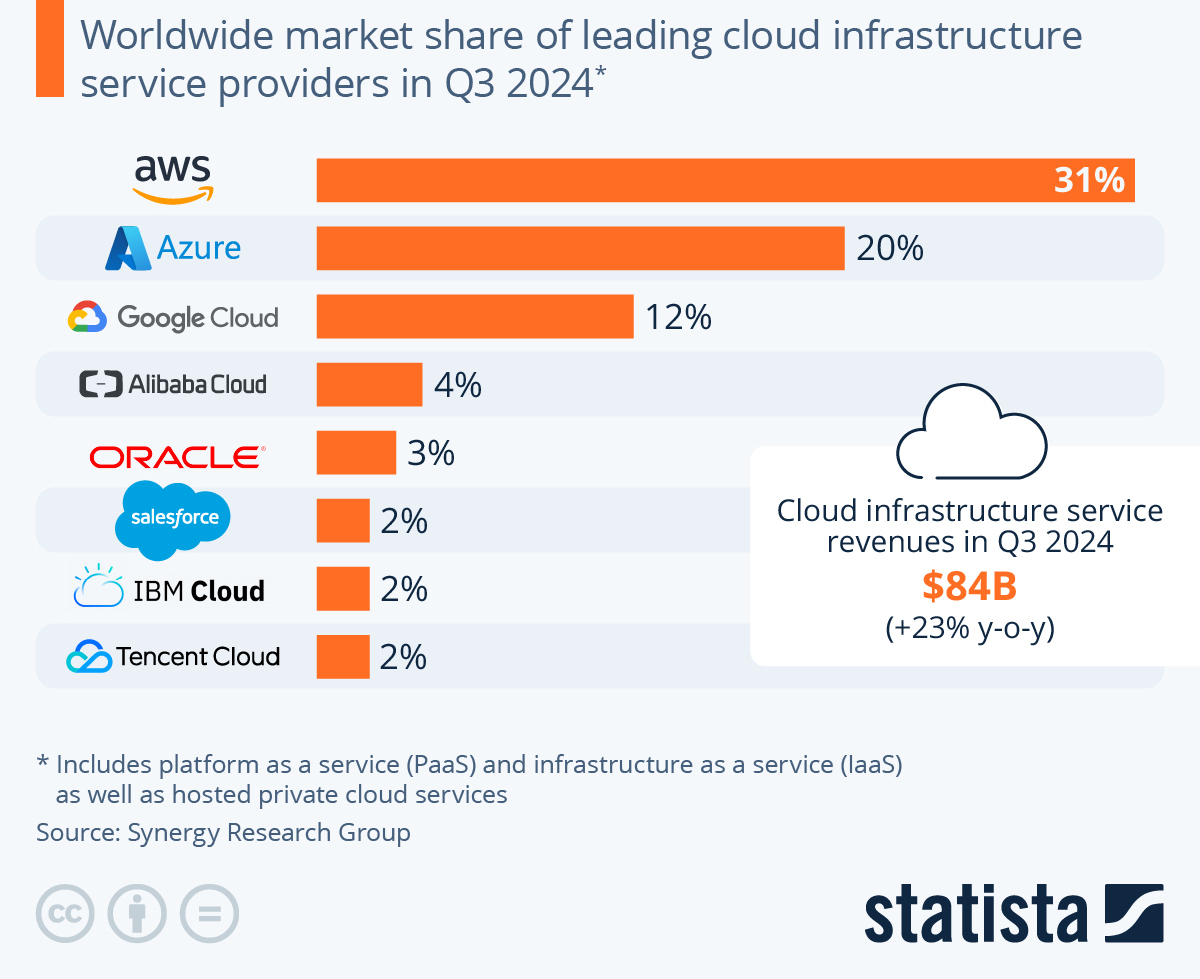
\includegraphics[width=0.75\linewidth]{images/pcp.jpeg}
    \caption{Worldwide market share of leading cloud infrastructure service providers as of Q3 2024 \cite{statista_cloud_market_share}}
    \label{fig:pcp}
\end{figure}
  
\subsection{Cloud Regions and Availability Zones}

With the term \textbf{cloud region}, cloud providers refer to a geographical area where they have one or more data centers.
Cloud providers usually further divide regions into availability zones (AZs) which main purpose is to provide high availability and fault tolerance.
For the purpose of this work, we will consider the concept of \textbf{cloud region} as the primary unit of deployment of cloud resources.
Usually, by cloud providers design choice, each cloud region supports only a subset of the available cloud services and instance types (virtual machines).
However, we could safely assume that our targeted workload specifications are quite standard and therefore can be scheduled on any cloud region.
As of late 2024, the three major cloud service providers have established extensive global infrastructures.
Table \ref{tab:cloud_regions_azs} shows the number of regions and availability zones (AZs) for each provider as of Q4 2024 - Q1 2025
\cite{statista_cloud_regions} \cite{aws_infrastructure}.
We must note that the number of regions and availability zones is constantly changing as cloud providers are expanding their global infrastructure.

\begin{table}[t]
    \centering
    \begin{tabular}{|l|c|c|}
    \hline
    \textbf{Cloud Provider} & \textbf{Regions} & \textbf{Availability Zones} \\
    \hline
    Amazon Web Services (AWS) & 36 & 114 \\
    \hline
    Microsoft Azure & 33 & 93 \\
    \hline
    Google Cloud Platform (GCP) & 40 & 121 \\
    \hline
    \end{tabular}
    \caption{Number of Cloud Regions and Availability Zones by Provider as of 2024 \cite{statista_cloud_regions}}
    \label{tab:cloud_regions_azs}
\end{table}

We must also note that each public cloud provider has a different number of regions and zones and also different naming conventions for them.
There is no standardization nor a convention in the industry for this and cloud providers have chosen their own naming schemes.
For instance, a region located in London is called ``\textit{eu-west-2}'' in AWS, ``\textit{uk-west}'' in Azure and ``\textit{europe-west2}'' in GCP.
This detail must be taken into account when designing and implementing a multi-cloud system.
For what concerns the geo-distribution of cloud regions, as an example, Figure \ref{fig:azure_data_centers} shows the location of \textbf{Azure cloud data centers} around the world and the country Grid Carbon Intensity as reported by Electricity Maps (year 2024) \cite{electricity_maps}.
The Grid Carbon Intensity is a measure of the carbon intensity of the electricity grid of a country and is expressed in grams of CO2 equivalent per kilowatt-hour (gCO2eq/kWh) and it is included in the figure to provide an insight on the carbon footprint of the cloud regions as it will be a key factor in the scheduling policy of our system.
Data center coordinates are retrieved by an Azure CLI command dump \cite{azure_data_centers_information} and plotted on a map using the Natural Earth dataset \cite{naturalearthdata}.

\begin{figure}[t]
    \centering
    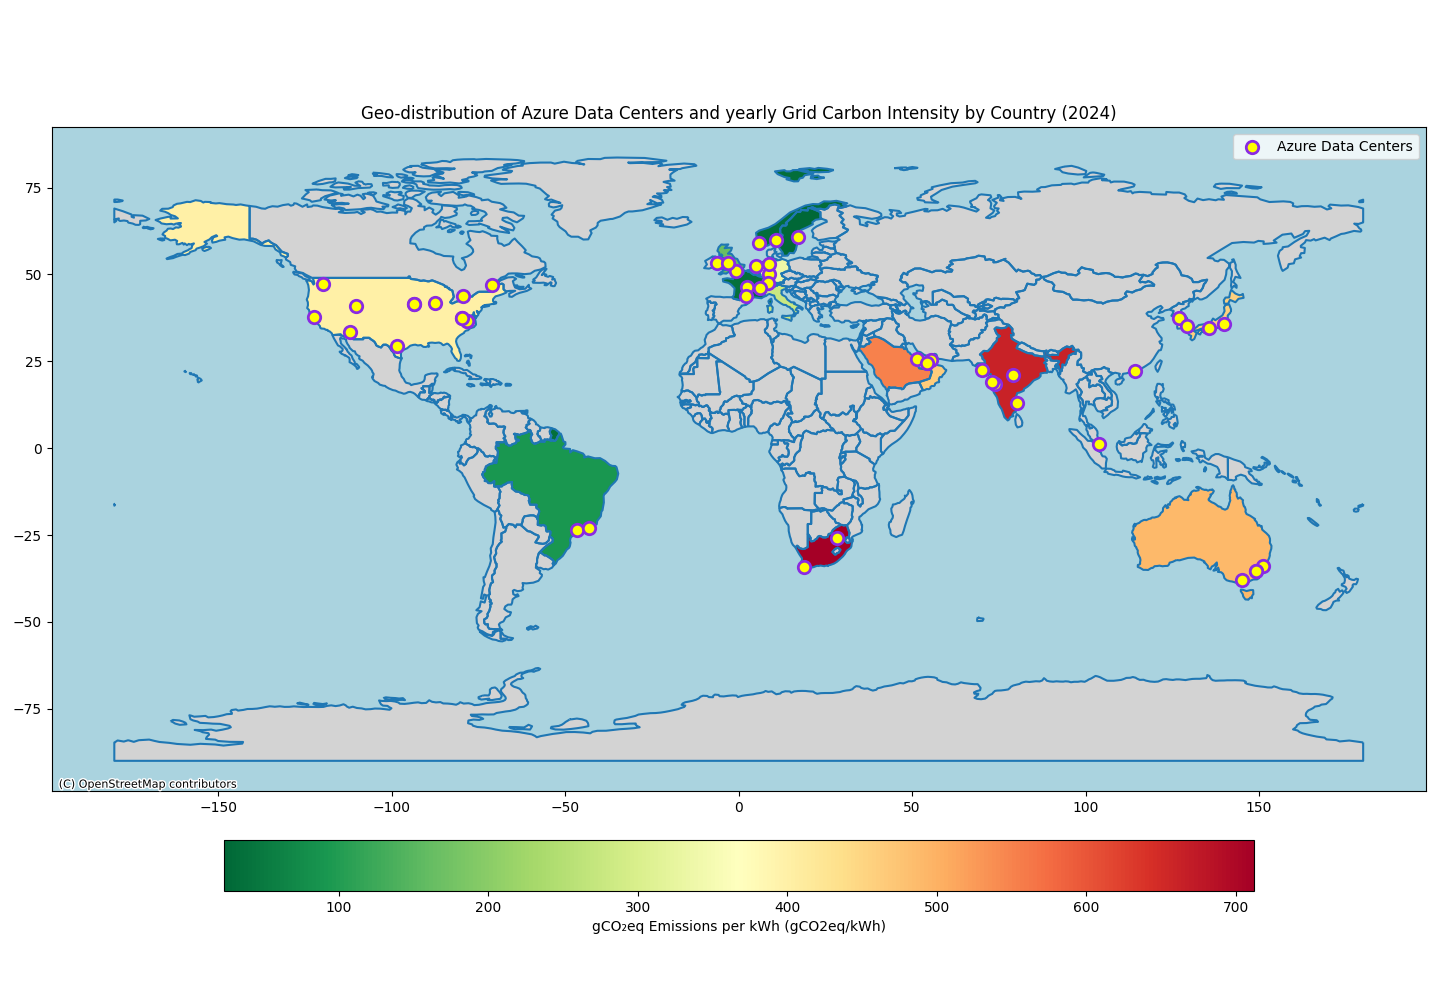
\includegraphics[width=1\linewidth]{images/azure_data_centers.png}
    \caption{Geo-distribution of Azure data centers with country Grid Carbon Intensity}
    \label{fig:azure_data_centers}
\end{figure}

\subsection{Multi-cloud paradigm}

The multi-cloud paradigm refers to the strategic utilization of cloud services from multiple public cloud providers within a single, heterogeneous architecture. 
This approach allows organizations to distribute workloads, applications, and data across multiple public cloud providers \cite{google_multicloud}.
On the other hand, the hybrid cloud paradigm refers to utilization of both public cloud services and on-premises infrastructure (e.g., a private cloud).
The multi-cloud strategy is often adopted by organizations to \textbf{avoid vendor lock-in}, \textbf{increase redundancy}, \textbf{increase flexibility} and \textbf{optimize costs} \cite{google_multicloud}.
For what concerns flexibility and optimization, a multi-cloud strategy allows an organization to select the best service on a case-by-case basis, leveraging the strengths of each provider.
Moreover, single point of failure weaknesses are mitigated by distributing workloads or critical services across multiple providers.
It could even be the case that, for the end user, the choice of the cloud provider for a service is transparent meaning that the organization itself (or the system) is the one that decides which cloud provider to use for a specific service based on some criteria.

To avoid vendor lock-in, applications must be designed to be \textbf{cloud-agnostic} and leverage open-source technologies (e.g., Kubernetes) and standards \cite{google_multicloud}.
If an application is designed to be cloud-agnostic, it can be relatively easily migrated from one cloud provider to another.
Multi-cloud is a strategy that might be more difficult to implement compared to a single cloud strategy but the long-term benefits are significant.

\textbf{Challenges} and \textbf{disadvantages} are also present in a multi-cloud strategy \cite{google_multicloud}.
As a matter of fact, it can be safely said that \textbf{complexity in the overall infrastructure management is increased}.
Another challenge is the \textbf{integration of services} across different cloud providers.
An additional consideration could be done in terms of security: a multi-cloud strategy can \textbf{increase the attack surface} of an organization, therefore increasing the requirement for security measures.
\newline
For the purpose of this work, adopting a multi-cloud strategy is beneficial for several reasons.
First and foremost, it achieves \textbf{user-centric flexibility} bringing the benefits described above.
If a user or organization has a preference for a specific cloud provider, the system can be configured to use only that provider or a specific subset of providers.
Secondly, the system can be designed to be \textbf{cloud-agnostic}, meaning that the choice of the cloud provider is transparent to the end user. 
With some specific configurations, the subset of providers to be used can be decided by the system itself based on some criteria.
Currently, as described in section \ref{sec:scheduling_outcome_policy}, the user can specify a subset of cloud providers (among the 3 major ones) to be used for the deployment of resources.
Finally, since different cloud providers have data centers in various locations around the world, some low-carbon regions might be available only on a specific cloud provider and this could be leveraged for the deployment of resources.

\section{GreenOps landscape}

GreenOps is the abbreviation for ``\textbf{Green Operations}" and is the term used to describe an operational model that aims to integrate sustainable practices into an organization's digital operations, with a particular focus on cloud computing and data centers.
The interest in GreenOps has been growing in the last years due to the increasing awareness of the environmental impact of data centers and cloud infrastructures.
%As a matter of fact according to various sources, the carbon footprint of data centers is [...]
The rising interest in the GreenOps ecosystem is also influenced by political and regulatory factors as the European Union's ambitious goals for the reduction of greenhouse gas emissions.
In particular, the \textit{Climate Neutral Data Centre Pact in Europe}, is an EU initiative which aims for making climate-neutral data centers by 2030 \cite{climate_neutral_data_centre_pact}.
Being the work of this thesis focused on the cloud ecosystem, we deem useful to cite the Technical Advisory Group (TAG) on Environmental Sustainability which is focused on the cloud-native sustainability landscape.
The TAG is part of the Cloud Native Computing Foundation (CNCF) and aims to provide guidance, standards, and best practices for the industry \cite{tag_env_sustainability}.

% https://hbr.org/2020/09/how-green-is-your-software
% https://www.usenix.org/publications/loginonline/slos-and-ghgs

\subsection{Green Software Foundation}

Another pivotal actor in the GreenOps landscape is the Green Software Foundation.
The Green Software Foundation is a non-profit organization, part of the Linux Foundation, that aims to promote the development of green software and to provide a set of standards, tooling and best practices for the industry \cite{green_software_foundation}.
It is considered useful to provide a quick summary of the foundation's major projects that are relevant to the context of this work.

\subsubsection{Software Carbon Intensity Specification}

Software Carbon Intensity Specification (SCI) is a specification that aims to provide a standard way to measure the carbon intensity of software systems.
SCI is defined as a rate: the amount of carbon emissions per one unit of $R$ where $R$ is a functional unit for the software system (e.g., API call, new user, DB query, etc.) \cite{sci}.

The SCI can be defined as follows:
\[
SCI = C \times R = (O + M) \times R = ((E \times I) + M) \times R
\]

where:
\begin{itemize}[itemsep=0.2pt, topsep=1pt]
    \item[$\bullet$] $SCI$ is the Software Carbon Intensity
    \item[$\bullet$] $C$ is the carbon emissions
    \item[$\bullet$] $R$ is the functional unit
    \item[$\bullet$] $O$ is the operational emissions
    \item[$\bullet$] $M$ is the embodied emissions
    \item[$\bullet$] $E$ is the energy consumption
    \item[$\bullet$] $I$ is the carbon intensity
\end{itemize}

\subsubsection{Real Time Cloud}
\label{sec:real_time_cloud}

The Real Time Cloud project aims to provide a standard for real-time carbon emissions data reporting for cloud providers.
The goal is to provide real-time access to information about cloud regions, power usage effectiveness (PUE), water usage effectiveness (WUE), carbon-free energy from the grid and from Cloud provider individual initiatives.
The concept is similar to FOCUS specification for FinOps \cite{finops_focus_spec} but is at a very early stage and is not yet adopted by cloud providers as of 2025 \cite{real_time_cloud}.

%https://github.com/Green-Software-Foundation/real-time-cloud?tab=readme-ov-file

\subsubsection{Impact Framework}
\label{sec:impact_framework}

The Impact Framework is a flexible framework for measuring and reporting the environmental impact of software systems \cite{impact_framework}.
The core of the framework is represented by a \textbf{Manifest file} which is a YAML file that is used both for describing \textbf{calculation pipelines} and for storing the results of the calculations.
Pre-built plugins are available for the most common calculations (e.g., carbon intensity, energy consumption, etc.) but custom plugins can be developed as well \cite{impact_framework}.
A potential integration of this framework with our system is described in section \ref{sec:impact_framework_integration}.

%https://patterns.greensoftware.foundation/catalog/cloud/choose-region-closest-to-users
%[which patterns are used in our system]

\subsection{Computational Sustainability by Public Cloud Providers}

For the purpose of ths work, we assume that a cloud data center will likely rely on the same energy sources that characterize a specific geographical region.
Indeed, cloud data centers typically draw power from their local electrical grids, meaning their carbon emissions are closely tied to the energy mix of their specific geographical regions just like any other industrial facility.
For instance, if Finland's energy production is characterized by low carbon emissions, data centers located there are likely powered by clean energy sources. 
However, some public cloud providers may implement individual initiatives to enhance their access to renewable energy or enhance their energy efficiency and by consequence to reduce their carbon footprints.
For instance, according to an AWS internal report, thanks to their works towards sustainability, they have been able to obtain an infrastructure that is up to 4.1 times more energy efficient than an equivalent on-premise infrastructure \cite{aws_sustainability}.
%what are they already doing
%improving energy efficiency by reducing their PUE
%(Power Usage Effectiveness (PUE) is the ratio of the total energy used by a data center to the energy used for computing.)
%what microsoft is already doing with alternative energy sources apart from grid
%https://blog.google/inside-google/infrastructure/data-centers-work-harder-sun-shines-wind-blows/
%Google CFE\%: “This is the average percentage of carbon free energy consumed in a particular location on an hourly basis, while taking into account the investments we have made in carbon-free energy in that location. This means that in addition to the carbon free energy that's already supplied by the grid, we have added carbon-free energy generation in that location”.
%When selecting a Google Cloud region, the user can see the carbon-free energy percentage (CFE\%) for that region.
%usually big companies leverage financial instruments like PPAs to buy renewable energy therefore their emissions are not zero but they are offset by the renewable energy they buy.
As another example of the efforts made by public cloud providers in the field of carbon-aware computing, we can describe how Google has been working on carbon-aware computing for internal use. 
In particular, they exploit workload flexibility to shift when, where and how computing is done to reduce carbon emissions \cite{google_carbon_aware_computing}.
Some of the types of workloads they identified as flexible are: \textbf{video processing}, \textbf{training large-scale machine learning models}, \textbf{simulation pipelines}.
The main components they recognized to be necessary for carbon-aware computing are: accurate carbon intensity data, scalable infrastructures and migrations mechanisms \cite{google_carbon_aware_computing}.
Another important point is to adopt a \textbf{data-driven methodology}.
Indeed, at Google the total amount of work (computing) that needs to get done per day is quite predictable thanks to the large amount of data they can analyze to make predictions \cite{google_carbon_aware_computing}.

In section \ref{sec:carbon_metrics} we will briefly describe how public cloud providers are already providing carbon footprint data reports to their customers.

\section{Kubernetes}

Kubernetes (K8s) is an open-source platform for automating the orchestration of containerized applications.
It is widely used in the industry and became the \textbf{de-facto standard for container orchestration}.
Figure \ref{fig:kubernetes_architecture} shows the Kubernetes architecture as described and depicted by the Cloud Native Computing Foundation (CNCF) \cite{kubernetes_cnfc}.

\begin{figure}[t]
    \centering
    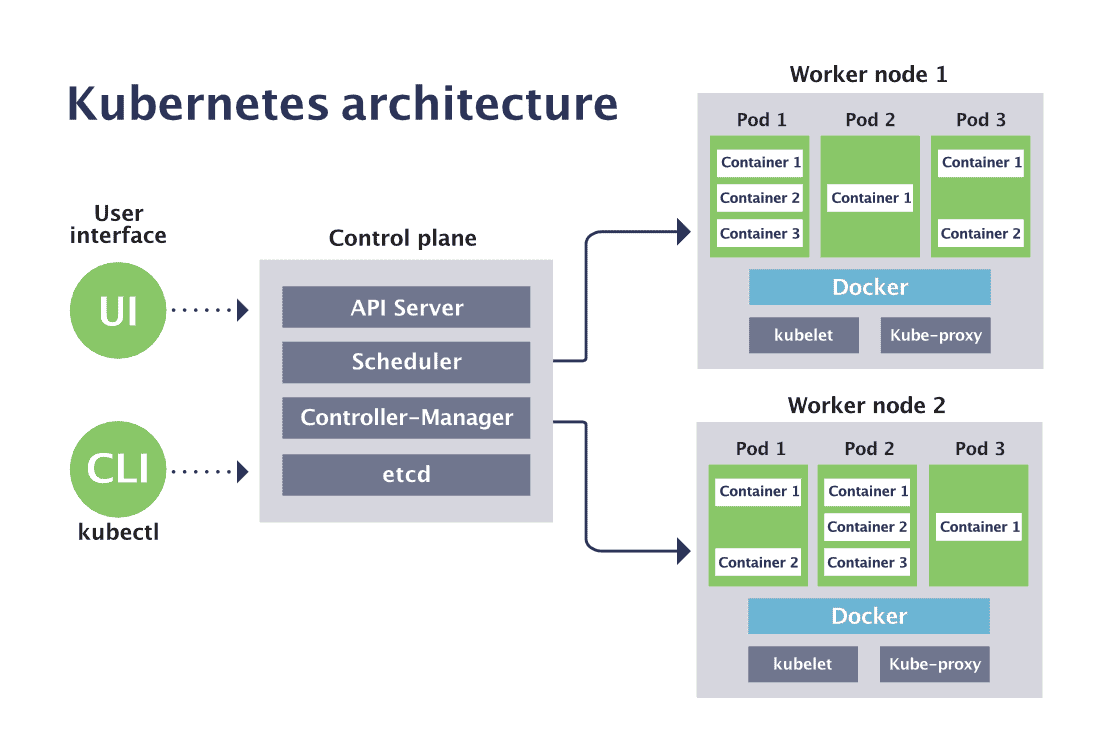
\includegraphics[width=1\linewidth]{images/kubernetes-architecture-diagram.png}
    \caption{Kubernetes architecture by CNCF \cite{kubernetes_cnfc}}
    \label{fig:kubernetes_architecture}
\end{figure}

The main components of Kubernetes are:
\begin{itemize}[itemsep=0.2pt, topsep=1pt]
    \item[$\bullet$] \textbf{API server}: the central component that manages the Kubernetes cluster. It exposes the Kubernetes API and is responsible for validating and mutating data related to Kubernetes objects before persisting them in the cluster state.
    \item[$\bullet$] \textbf{etcd}: a key-value store used to store the cluster state.
    \item[$\bullet$] \textbf{Controller manager}: a daemon that embeds the core control loops shipped with Kubernetes.
    \item[$\bullet$] \textbf{Scheduler}: a component that assigns Pods to nodes.
    \item[$\bullet$] \textbf{Kubelet}: an agent that runs on each node in the cluster. It makes sure that containers are correctly running in Pods.
    \item[$\bullet$] \textbf{Proxy}: a network proxy that runs on each node in the cluster. It maintains network rules and it is responsible for routing network traffic.
    \item[$\bullet$] \textbf{Container runtime}: the software that is responsible for running containers on the Node (in this case represented by Docker but other runtimes like containerd are supported).
\end{itemize}

The first four components of the above list are the main control plane components of Kubernetes while the last three are the main components of each worker node in the cluster.
It must be noted that in our system we are not extending the Kubernetes scheduler as described in sections \ref{sec:low_carbon_k8s_scheduler} and \ref{sec:microsoft_carbon_aware_k8s}, since we are not dealing with the scheduling of in-cluster resources (e.g., Kubernetes Pods) nor with the provisioning of entire Kubernetes clusters.
We are instead focusing on the \textbf{management of external resources on cloud providers}, leveraging Kubernetes as a control plane for the management of these resources.
As described in the following section, our focus will be on the Kubernetes API server and in particular on Kubernetes admission control.

\subsection{Kubernetes extensibility}
\label{sec:kubernetes_extensibility}

% https://www.cncf.io/blog/2022/06/15/kubernetes-operators-what-are-they-some-examples/

Kubernetes allows for the extension of its functionalities through the use of \textbf{Custom Resource Definitions (CRDs)} and \textbf{Kubernetes Operators}, effectively adopting the so-called \textbf{operator paradigm}.
Simply put, CRDs are a way to instruct Kubernetes to manage new resource types and can be added and removed from a Kubernetes cluster at runtime, through dynamic registration.
They are a \textbf{schema} that defines the structure of the resource and the Kubernetes API server will validate the resource against the schema.
\textbf{Custom Resources (CRs)} are actually instances of the resources defined by CRDs and are managed by an operator.
An operator is a special type of controller tasked with managing the lifecycle of the CRs.
Indeed they implement \textbf{control loops} to compare the \textbf{current state} of the resources they manage with the \textbf{desired state} and take actions to make the current state converge to the desired state.
A high-level overview of the operator paradigm is depicted in Figure \ref{fig:operator_paradigm}.
Effectively, the code of an operator is usually deployed on the Kubernetes cluster in the form of a Kubernetes deployment.
This concept is similar to the standard built-in Kubernetes resources which are however manged by built-in controllers (e.g., Deployment controller, ReplicaSet controller, part of Kubernetes controller manager).

\begin{figure}[t]
    \centering
    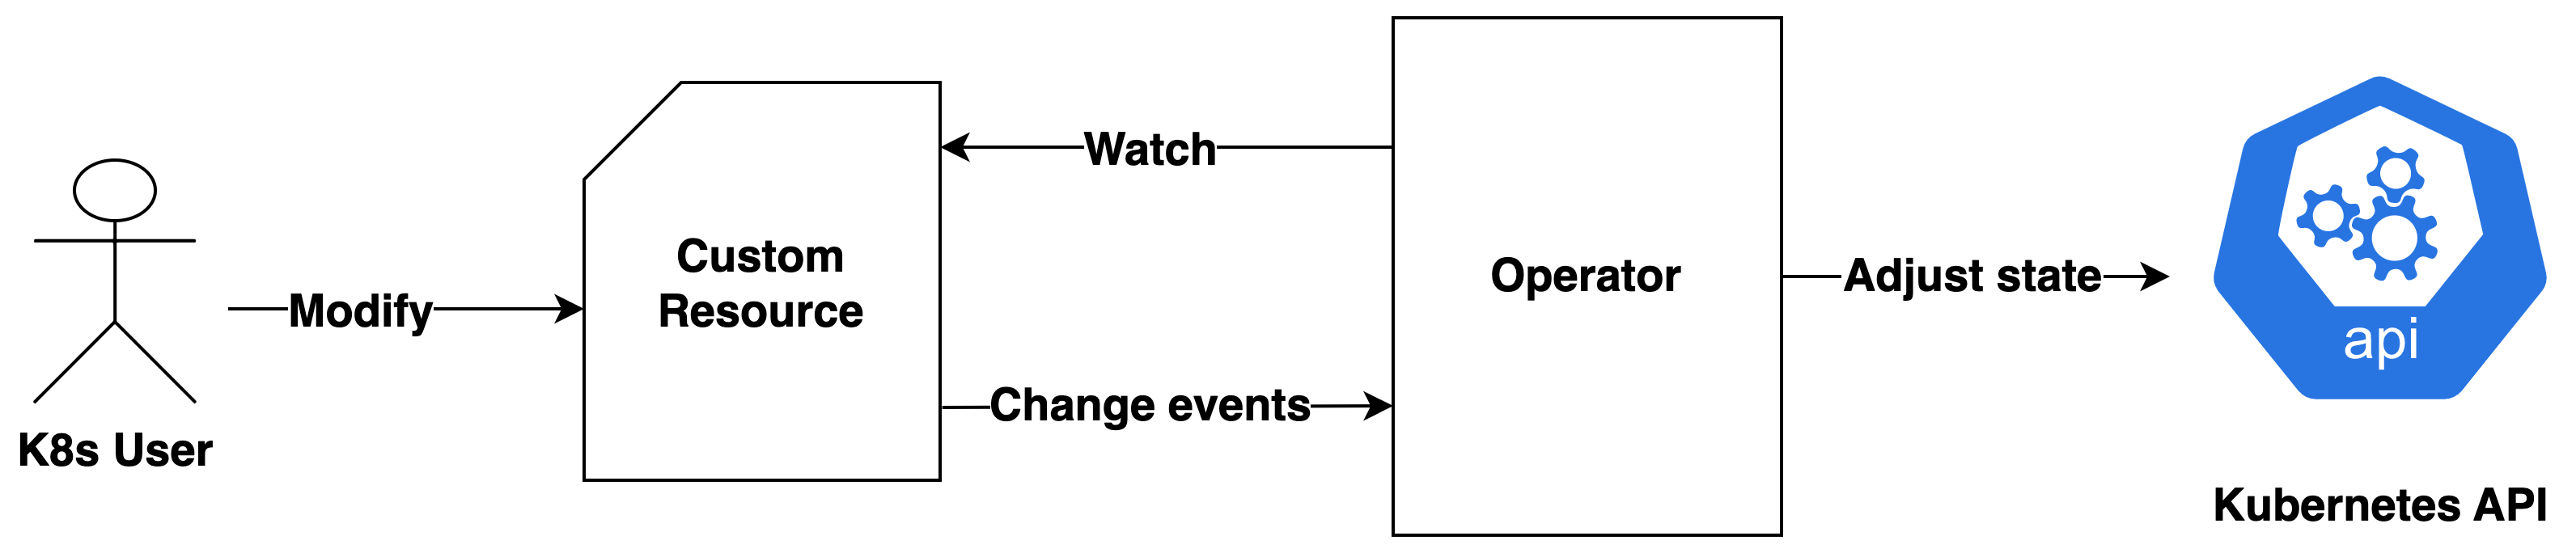
\includegraphics[width=1\linewidth]{images/opeartor_paradigm.png}
    \caption{Operator paradigm}
    \label{fig:operator_paradigm}
\end{figure}

\subsection{Kubernetes as a platform}

Recently, the paradigm of leveraging Kubernetes as a platform to manage external resources has become more and more popular.
Therefore, Kubernetes use cases have expanded beyond the management of containerized applications to the management of any desired resource on any infrastructure.
The idea is to \textbf{represent external resources as Kubernetes objects} and leverage Kubernetes' declarative paradigm and robust API to achieve unified and efficient infrastructure management.
This approach can be exemplified by the public cloud providers' operators which extend Kubernetes to manage their cloud resources as described in section \ref{sec:cloud_providers_operators}.

For instance, Config Connector is a Kubernetes operator developed by Google Cloud that allows to configure numerous Google Cloud services and resources using Kubernetes tooling and APIs \cite{gcp_config_connector}.
The general idea is that organizations might have to deal with a \textbf{heterogeneous infrastructure} composed of different cloud providers and on-premises resources. 
By \textbf{unifying infrastructure management under Kubernetes}, complexity is reduced and velocity is increased because the same tools and APIs can be used to manage all the resources in a consistent way \cite{gcp_config_connector}.
In particular, Config Connector provides a set of CRDs that represent Google Cloud resources and services (e.g., Google Compute Instances, Google Kubernetes Engine clusters, BigQuery datasets, etc.) and the Config Connector operator is responsible for managing the lifecycle of these resources.

% https://aws.amazon.com/it/blogs/containers/kubernetes-as-a-platform-vs-kubernetes-as-an-api-2/

\subsection{Helm}

Helm is the de-facto standard \textbf{package manager} for Kubernetes and it allows to define, install and manage applications in a simpler way compared to standard resource manifests \cite{helm}.
The key concept is the \textbf{Helm chart}, which is a collection of files that describe a related set of Kubernetes resources. 
These files are mainly of two types: templates and values.
The \textbf{templates} are Kubernetes manifest files that are rendered by Helm's \textbf{powerful templating engine}. 
The \textbf{values} are the set of variables that are used to render the templates.
Upon a chart installation, Helm will render the templates ``injecting" the values and deploying the resources in the Kubernetes cluster. 
One major advantage that Helm provides is the complete management of the lifecycle of the resources.
As a matter of fact, Helm allows to easily \textbf{upgrade}, \textbf{rollback} and \textbf{uninstall} the Kubernetes resources deployed with a Helm chart reducing time and human errors in such operations \cite{helm}. 
Without Helm, the user would have to deal with each single Kubernetes resource manifest file and manually apply changes to them.
Finally, users can benefit of Helm charts already developed by the community and leverage chart distribution within their organization using Helm repositories (either public or private).

\section{Krateo PlatformOps}
\label{sec:krateo}

Krateo PlatformOps (Krateo) is an \textbf{open-source Kubernetes-based platform} that aims to provide a unified interface for managing any desired resource on any infrastructure \cite{krateo_docs}.
Krateo runs as a Kubernetes deployment inside a Kubernetes cluster but \textbf{acts as a control plane} even for resource external to the Kubernetes cluster.
The only requirement for this management is that the resources need to be logically ``encoded'' using a YAML file which represents the desired state of the resources \cite{krateo_docs}. \newline
% Platform engineering
% Developer platform: a unified environment providing tools, services, and infrastructure that enables teams to efficiently build, test, and deploy software without managing underlying complexity. This complexity is handled by the platform team.
% Recognized by Gartner. Gartner said ... by 2025 companies without a ... (cite)
Krateo has three main components:
\begin{itemize}[itemsep=0.2pt, topsep=1pt]
    \item[$\bullet$] Krateo Composable Operations: a set of core modules needed for resource managment
    \item[$\bullet$] Krateo Composable Portal: a web-based declarative user interface
    \item[$\bullet$] Krateo Composable FinOps: a set of modules for advanced cost optimization
\end{itemize}

For the purpose of this work, we will focus on the \textbf{Krateo Composable Operations} part, which is the core of the Krateo platform and is responsible for managing the lifecycle of resources in a Kubernetes cluster \cite{krateo_docs}.
Krateo Composable Operations is composed in turn by several components. 
Due to their core importance in our system, we will briefly describe the functionalities of the \textbf{Krateo core-provider} and the \textbf{Krateo composition-dynamic-controller} as described in Krateo's official documentation \cite{krateo_core_provider}, \cite{krateo_composition_dynamic_controller}.

\subsection{Krateo core-provider}

The Krateo core-provider, as its name suggests, is the core component of the Krateo platform.
It is a \textbf{Kubernetes operator} that has the duty of downloading and managing Helm charts. 

It first checks for the existence of a file named \textit{values.schema.json} in the chart folder and uses it to generate a Kubernetes CRD, accurately representing the possible values that can be expressed for the installation of the chart \cite{krateo_core_provider}.
The file \textit{values.schema.json} is a JSON schema that describes the structure of the \textit{values.yaml} file for the related Helm chart and it is considered a standard best practice for Helm charts. 
It basically provides a way to validate the \textit{values.yaml} file before the Helm chart is installed (i.e., to check if the values are in the correct format and if all the required values are present) \cite{krateo_core_provider}.
Therefore, generally speaking, the file \textit{values.schema.json} could be useful in the context of DevOps practices and CI/CD pipelines but in the case of Krateo it is pivotal for the generation of the CRD.
In other words, the Krateo core-provider operator is responsible for deploying the Helm chart as a \textbf{native Kubernetes resource}, which allows for the management of the whole Helm chart lifecycle through Kubernetes APIs \cite{krateo_core_provider}.
As a matter of fact, out of the box, Kubernetes does not provide a way to manage Helm charts natively and the Krateo core-provider is one tool that allows to do so.

Krateo core-provider introduces a Kubernetes CRD introduced called \textbf{\textit{CompositionDefinition}} to represents the Helm chart and its values (a Helm Chart archive with a JSON Schema for the \textit{values.yaml} file) \cite{krateo_core_provider}.
Upon a CompositionDefinition manifest application to the Kubernetes cluster, the Krateo core-provider generates the CRD from the schema defined in the \textit{values.schema.json} file included in the chart. 
It then deploys an instance of the Krateo composition-dynamic-controller, configuring it up to manage resources of the type defined by the CRD \cite{krateo_core_provider}.
This is another example of the operator paradigm described in section \ref{sec:kubernetes_extensibility} where the Krateo core-provider is the operator and the CompositionDefinition is the CRD.

\subsection{Krateo composition-dynamic-controller}

The Krateo composition-dynamic-controller (CDC) is the Kubernetes operator that is instantiated by the Krateo core-provider to manage the specific CRs whose CRDs are generated by the core-provider.
In practice, when a CR is created, the specific instance of Krateo composition-dynamic-controller checks if a Helm release associated with the CR already exists in the cluster \cite{krateo_composition_dynamic_controller}. 
If this is not the case, it performs an \textit{helm install} operation using the values specified in the CR to create a new Helm release. 
This will practically deploy all the resources defined in the Helm chart (in the folder ``/templates'') using \textbf{Helm's templating engine}.
This feature is particularly important in the context of the system described in this thesis and in particular for multi-cloud resource management as explained in section \ref{sec:krateo_integration}.
However, if the Helm release does already exist, it instead executes an \textit{helm upgrade} operation, updating the release's values with those specified in the CR, effectively updating the resources in the cluster.
This mechanism will be leveraged as well for a particular feature  of our system (i.e., ``waiting logic'') described in section \ref{sec:scheduling_time_waiting_logic}.
Finally, if and when the CR is deleted from the cluster, the instance of the Krateo composition-dynamic-controller performs an \textit{helm uninstall} on the Helm release, effectively removing all the resources defined in the Helm chart from the cluster \cite{krateo_composition_dynamic_controller}. \\

It must be said that Krateo composition-dynamic-controller has a set of additional features that are not described in this work such as multi-version support.
Figure \ref{fig:krateo_core_provider} shows the architecture of the Krateo core-provider and Krateo composition-dynamic-controller, as described and depicted in \cite{krateo_core_provider}.

\begin{figure}[t]
    \centering
    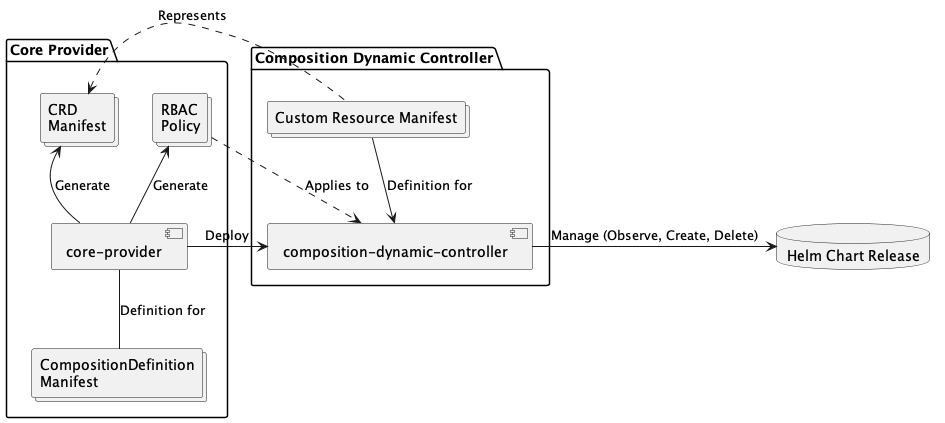
\includegraphics[width=1\linewidth]{images/kraeto_core_provider.png}
    \caption{Krateo core-provider and composition-dynamic-controller architecture \cite{krateo_core_provider}}
    \label{fig:krateo_core_provider}
\end{figure}

\section{Open Policy Agent}

Open Policy Agent (OPA) is an open-source general-purpose \textbf{policy engine} that enables unified policy decision-making across several types of environments \cite{opa_docs}. 
OPA provides a declarative language called \textbf{Rego} enabling a paradigm known as ``\textbf{Policy as Code}" \cite{opa_docs}.
Open Policy Agent can be integrated as a sidecar container, host-level daemon, or library to perform policy decisions for a plethora of use cases: \textbf{Kubernetes admission control}, CI/CD pipelines, container images, microservices, etc.\cite{opa_docs}. 

\subsection{Policy as Code paradigm}

According to AWS, Policy as Code (PaC) is a software automation approach which is similar to Infrastructure as Code (IaC) \cite{pac_aws}. 
PaC helps assess company system configurations and validate compliance requirements through software automation \cite{pac_aws}. 
The perceived value of this type of automation in the software development lifecycle has grown significantly in modern enterprises. 
This large adoption is probably driven by the inherent consistency and reliability it provides, ensuring standardized enforcement of policies and reducing human error, as what happened with the IaC approach \cite{pac_aws}.

OPA's generic definition of policy is: ``\textit{A policy is a set of rules that governs the behavior of a software service}" \cite{opa_philosophy}. OPA provides a high-level declarative language called \textbf{Rego} to define policies in a flexible manner. 
One of OPA's key strengths is its \textbf{domain-agnostic design}, allowing it to enforce policies across various systems and environments. 
This makes it highly adaptable to different use cases, ranging from access control to infrastructure security. 
Some representative examples of policies that OPA can enforce include:

\begin{itemize}[itemsep=0.2pt, topsep=1pt]
    \item[$\bullet$] Restricting which specific image registries can be used for deploying new pods in a Kubernetes cluster.
    \item[$\bullet$] Controlling whether a specific user is permitted to perform delete operations on certain resources on an API server.
    \item[$\bullet$] Enforcing network security policies, such as blocking external access to sensitive internal services.
    \item[$\bullet$] Ensuring cloud infrastructure compliance, for example, by verifying that new cloud resources to be provisioned follow predefined security configurations.
    \item[$\bullet$] Enforcing that new deployed servers must have the prefix ``server-" in their name.
\end{itemize}

Another interesting example is the use of OPA for \textbf{compliance automation for AWS infrastructure} \cite{10612535}. 
In this case, OPA is used by the authors as a step in a CI/CD pipeline to enforce compliance policies on AWS infrastructure represented with the IaC tool CloudFormation \cite{10612535}.
Therefore, the use cases covered span from role-based access control to container image security and beyond.
\newline

Another important aspect of OPA is that it effectively \textbf{decouples} policy decision-making from policy enforcement \cite{opa_docs}.
In practice, this means that when a software module needs to make a policy decision, it queries OPA, supplying relevant data as input. 
In other words, policy decisions are \textbf{offloaded} to OPA rather than being hardcoded within individual services. 
This approach offers several key advantages \cite{opa_docs}:
\begin{itemize}[itemsep=0.2pt, topsep=1pt]
  \item[$\bullet$] \textbf{Centralized policy management}: policies are defined in a single location, ensuring uniform enforcement across all services of an organization.
  \item[$\bullet$] \textbf{Improved maintainability}: updating policies does not require modifying, recompiling or redeploying application code, reducing complexity, errors and deployment overhead.
  \item[$\bullet$] \textbf{Greater flexibility}: policies can be dynamically updated (e.g., with CI/CD approaches) based on evolving security and compliance requirements. 
  \item[$\bullet$] \textbf{Scalability}: since OPA and application modules requiring policy decisions are not tightly coupled.
\end{itemize} 

\subsection{OPA Gatekeeper}

OPA Gatekeeper is a Kubernetes-native tool that extends OPA with \textbf{Custom Resources} and controllers to enforce policies within a Kubernetes cluster \cite{opa_gatekeeper}. 
As a matter of fact, it provides a declarative approach to defining and enforcing policies using Kubernetes Custom Resources. 
This makes it a convenient choice for simple and standard policy enforcement scenarios in Kubernetes, such as RBAC (Role-Based Access Control), basic security compliance, and resource constraints \cite{opa_gatekeeper}.
However, while OPA Gatekeeper is \textbf{well-suited for simple use cases}, it presents heavy \textbf{limitations} when addressing complex policy requirements, particularly when policies involve \textbf{mutations} or require access to \textbf{external data sources} \cite{opa_gatekeeper_external_data}. 
Indeed, these limitations make it unsuitable for the specific challenges tackled in this system. 
Therefore, after an initial investigation and Proof of Concept implementation, we decided to use a standard OPA server for policy enforcement mainly due to the flexibility it provides in handling diverse scenarios.
To illustrate the differences between a standard OPA policy and an OPA Gatekeeper policy, we present two examples:  
\begin{itemize}[itemsep=0.2pt, topsep=1pt]
  \item[$\bullet$] a simple Rego policy that enforces a basic constraint on Pod creation in a Kubernetes cluster.
  \item[$\bullet$] the corresponding policy implemented as an OPA Gatekeeper \textbf{ConstraintTemplate} and \textbf{Constraint} Kubernetes custom resources.
\end{itemize}

The first example demonstrates a standalone Rego policy, which can be evaluated directly by an OPA instance. 
While this approach is flexible and allows for fine-grained policy definition, it requires manual integration into the system, including policy distribution and enforcement setup.  

\begin{lstlisting}[language=rego, caption={Simple OPA Rego Policy}, label={lst:opa-rego}]
package kubernetes.admission

deny[msg] {
  input.request.kind.kind == "Pod"
  input.request.object.metadata.namespace == "restricted"
  msg := "Pods cannot be created in the 'restricted' namespace."
}
\end{lstlisting}

The second example, illustrated in listing \ref{lst:gatekeeper-template} utilizes OPA Gatekeeper and therefore its CRs. By using a ConstraintTemplate CR, policies can be enforced with Kubernetes tooling, making them easier to distribute and manage in this context.
In other words, with this kind of setting, OPA policy bundles are not employed in the same way as in the standard OPA server. Instead, policies are defined as Kubernetes resources, allowing for more straightforward policy enforcement and management within a Kubernetes environment.

\vspace{5cm}
\begin{lstlisting}[language=yaml, caption={OPA Gatekeeper ConstraintTemplate}, label={lst:gatekeeper-template}]
apiVersion: templates.gatekeeper.sh/v1
kind: ConstraintTemplate
metadata:
  name: podnamespaceconstraint
spec:
  crd:
    spec:
      names:
        kind: PodNamespaceConstraint
  targets:
    - target: admission.k8s.gatekeeper.sh
      rego: |
        package kubernetes.admission
        deny[msg] {
          input.review.object.metadata.namespace == "restricted"
          msg := "Pods cannot be created in the 'restricted' namespace."
        }
\end{lstlisting}

\begin{lstlisting}[language=yaml, caption={OPA Gatekeeper Constraint}, label={lst:gatekeeper-constraint}, float=htpb]
apiVersion: constraints.gatekeeper.sh/v1beta1
kind: PodNamespaceConstraint
metadata:
  name: restrict-namespace
spec:
  match:
    kinds:
      - apiGroups: [""]
        kinds: ["Pod"]
  parameters: {}
\end{lstlisting}

In the example, the policy is defined as a ConstraintTemplate, which is then instantiated as a Constraint Custom Resource of kind defined in the ConstraintTemplate. 
The ConstraintTemplate specifies the Rego policy logic, while the Constraint defines the target resources and parameters for policy enforcement. Therefore a ConstraintTemplate can be used by multiple Constraints, allowing for policy reuse.

OPA Gatekeeper also provides additional Kubernetes Custom Resources called \textit{mutators} (Assign, AssignMetadata, AssignImage, ModifySet) that allow modifying resource fields without writing Rego code \cite{opa_gatekeeper}. 
These mutators are useful for simple transformations, such as setting default labels or annotations. However simultaneous mutation of multiple fields leveraging external data is not supported \cite{opa_gatekeeper_external_data}. 
This limitation, in the context of our system, determined the choice of the standard OPA server for policy enforcement. \newline

It must be noted that OPA Gatekeeper limitations could be potentially addressed in future releases, making it a more viable option for complex policy enforcement scenarios. 
However, for the current system requirements, the standard OPA server was deemed more suitable due to its flexibility.

\section{MLflow}

MLflow is an open-source platform designed to facilitate and enhance the overall machine learning lifecycle. 
In particular, it offers tooling for \textbf{experiment tracking}, \textbf{model management}, and \textbf{model storage} \cite{mlflow_docs}.
It is compatible with various ML frameworks, including scikit-learn, PyTorch, TensorFlow, and XGBoost.
In particular, in the case of our system, PyTorch is the ML framework used for the forecasting models making MLflow a suitable choice for model management.
For what concerns model deployment, MLflow does not provide a built-in solution, but it is compatible with other tools like KServe which will be described in section \ref{sec:kserve}.

\subsection{MLflow Tracking Server}
\label{sec:mlflow_tracking_server}

MLflow Tracking Server is the central component of the MLflow platform which is responsible for logging and storing model training data, parameters, and metrics. 
It enables machine learning practitioners (e.g., data scientists, machine learning engineers) to track experiments, compare results, and reproduce models easily in a collaborative environment.
MLflow Tracking Server revolves around the concepts of \textbf{experiments}, which are collections of \textbf{runs}. 
Each run represents a single model training session, and it contains information such as parameters, metrics, and artifacts (e.g., model files).
Selected models can then be registered in the MLflow Model Registry, which is essentially an optional subset of the selected models that are ready for deployment.
Model selection can done with the aid of a user interface that allows ML practitioners to visualize and compare the results of different experiments, making it easier to select the best model for deployment.
MLflow Tracking Server, as the name suggest, is a server that is constantly waiting for new data to be logged. 
Said data comes from the various training scripts that are executed by the data scientists or machine learning engineers which are run in  training environments.
In particular the training scripts must be instrumented with the \textbf{MLflow API calls} to log the data in the remote MLflow Tracking Server.
This setting is very flexible since the training scripts can be run in any environment (e.g., local environment, Universities' HPC clusters), as long as they have access to the MLflow Tracking Server.
It is deemed important to mention some of the MLflow API calls that are used in the training scripts: the \textit{infer\_signature} and \textit{autolog} functions \cite{mlflow_docs}.
The \textit{infer\_signature} function captures the \textbf{input and output schema of the model}, which is important for the deployment of the model.
The \textit{autolog} function is used to automatically log the parameters and metrics of the model training session, without the need to manually log them. In particular, each supported ML framework has its own autolog function which is used to automatically log the parameters and metrics of the model training session.
The final phase of a model training session is the automatic creation of a \textbf{self-contained directory}, named after the experiment and run IDs, that contains all the necessary files to deploy the model. 
In particular, the folder contains: the serialized model with model weights, the configuration files (\textit{conda.yaml}, \textit{requirements.txt}), and the \textit{MLmodel} file that contains additional configuration, among which, the model signature.
The self-contained folder is then automatically uploaded to the MLflow Tracking Server as an artifact.
The following is an example of the structure of the self-contained directory created by MLflow after a PyTorch model training session: \\

\dirtree{%
.1 model/.
.2 MLmodel.
.2 conda.yaml.
.2 python\_env.yaml.
.2 requirements.txt.
.2 data/.
.3 model.pth.
.3 pickle\_module\_info.txt.
}

\section{KServe}
\label{sec:kserve}

KServe is an open-source model inference platform that extends Kubernetes with a set of CRDs to \textbf{deploy} and scale machine learning models in production environments \cite{kserve_docs}.
KServe can be deployed in several ways, one of which is the ``\textit{Serverless mode}'' which is built on top of Istio and Knative, leveraging their powerful capabilities such as automatic scaling. 
There are two main CRs that can be used to set up a model serving environment: \textit{\textbf{ServingRuntimes}} (or \textit{\textbf{ClusterServingRuntimes}}) and \textit{\textbf{InferenceServices}} \cite{krateo_docs}.
The former are abstractions that define model serving environments, specifying the templates for Kubernetes Pods capable of serving particular model formats. 
The latter are actually leveraging the available ServingRuntimes to deploy the models in the system.  
KServe provides several out-of-the-box ClusterServingRuntimes for common model formats, such as TensorFlow, PyTorch, and XGBoost, which can be used to deploy models without the need to define and configure the runtimes themselves.

\subsection{Open Inference Protocol}

Interoperability is key in a fast-moving environment as the one of machine learning and AI. 
Therefore KServe has introduced the \textbf{Open Inference Protocol specification} to standardize the communication between inference servers and clients. 
The Open Inference Protocol has been adopted by several inference servers, including NVIDIA's Triton and Seldon MLserver \cite{kserve_oip}.
As mentioned in the previous section, the InferenceService CRs used in the system are leveraging the ``kserve-mlserver" ClusterServingRuntime, which under the hood uses MLserver that is compliant with the Open Inference Protocol.
The list of API endpoints specified by the Open Inference Protocol is shown in Table \ref{tab:oip_endpoints}.

\begin{table}[t]
\centering
\begin{tabular}{|l|l|l|}
\hline
\textbf{API}    & \textbf{Verb} & \textbf{Path}                                                                                         \\ \hline
Inference       & POST          & v2/models/{[}/versions/\textless{}model\_version\textgreater{}{]}/infer                               \\ \hline
Model Ready     & GET           & v2/models/\textless{}model\_name\textgreater{}{[}/versions/{]}/ready                                  \\ \hline
Model Metadata  & GET           & v2/models/\textless{}model\_name\textgreater{}{[}/versions/\textless{}model\_version\textgreater{}{]} \\ \hline
Server Ready    & GET           & v2/health/ready                                                                                       \\ \hline
Server Live     & GET           & v2/health/live                                                                                        \\ \hline
Server Metadata & GET           & v2                                                                                                    \\ \hline
\end{tabular}
\caption{Open Inference Protocol API endpoints specification \cite{kserve_oip}}
\label{tab:oip_endpoints}
\end{table}

\section{Cloud resource metrics}

% https://dynamorio.org/google_workload_traces.html

Metrics are data points that provide information about a system.
This information could be related to performance, behavior, resource utilization or any other aspect of the system that could be relevant.
In the context of cloud resource management, metrics are essential for monitoring the \textbf{performance and health of cloud resources}, enabling organizations to make informed decisions about resource allocation, scaling, and optimization.
Focusing on the first use case of the proposed system (i.e., VM scheduling for carbon footprint optimization), carbon metrics could be used to determine the carbon footprint of a scheduled VM.
How to measure the carbon footprint of a resource managed in the cloud is a complex and challenging task.
The carbon footprint of a cloud resource is influenced by several factors, such as the power usage effectiveness of the data center where the resource is hosted, the carbon intensity of the electricity grid in the region where the data center is located, whether the data center uses additional energy sources off the grid, and finally the energy consumption of the resource itself.
The last factor is probably the most difficult to measure, as a cloud resource is an \textbf{entity that is abstracted from the physical infrastructure}, and therefore it is not straightforward to measure its power consumption. 
In this first iteration of the system we are dealing for instance with virtual machines (VMs).
On the other hand, an on-premises server, for instance, could be potentially equipped with physical sensors that measure the direct power consumption of the server, but this is not the case for any cloud resource, especially since this work is focused on the consumer side of the cloud, where the consumer does not have access to any physical infrastructure.
Moreover, public cloud providers do not provide fine grained and real-time data about the carbon footprint of a resource, as they do not adhere yet to a common standard for carbon footprint calculation (e.g., Real Time Cloud proposed by the Green Software Foundation), like they instead do for the FOCUS standard for FinOps \cite{finops_focus_spec}.
In this section we want to give an brief overview of several metrics and methodologies that can be used \textbf{estimate the carbon footprint of a cloud resource}.
In addition, we will also discuss the \textbf{challenges and limitations} that can be encountered when dealing with this kind of task.

\subsection{System performance metrics}

System performance metrics are a category of metrics that provide information about the health and performance of a system.
Usually these metrics are related to bare-metal servers or virtual machines.
Other cloud resources that have a higher level of abstraction (e.g., containers, Kubernetes Pods, serverless functions) may expose a slighlty different set of metrics that fall into this category as well.
This category of metrics are also useful for the ``\textbf{day 2 operations}'', which are operations that are performed after the resource has been deployed and monitored for a certain period of time, briefly described in section \ref{sec:day2_operations}.

System performance metrics comprise, for instance:
\begin{itemize}[itemsep=0.2pt, topsep=1pt]
  \item[$\bullet$] CPU usage
  \item[$\bullet$] Memory usage
  \item[$\bullet$] Disk usage
  \item[$\bullet$] Network usage
  \item[$\bullet$] Processes related metrics \\
\end{itemize}

A standard strategy to collect these metrics is to use \textbf{agents} that are directly installed on the VMs and operate at the Operating System level.
Some examples of this kind of agents are the \textbf{Prometheus Node exporter} and the \textbf{Prometheus Process exporter}.
Figure \ref{fig:prometheus} shows an example of a standard Prometheus architecture used to collect system performance metrics using the Node exporter and the Process exporter on a set of Linux VMs.
In particular, the Node exporter collects metrics such as CPU usage, memory usage, disk usage, and network usage, while the Process exporter collects metrics about the various processes running on the VM (e.g., CPU and memory usage per process group).
Metrics are pulled by the Prometheus server, which stores them in a time-series database and makes them available for querying and visualization (e.g., using Grafana). 
In addition, the Prometheus server can be configured to send alerts based on the collected metrics leveraging the Alertmanager component. \newline

\begin{figure}[t]
  \centering
  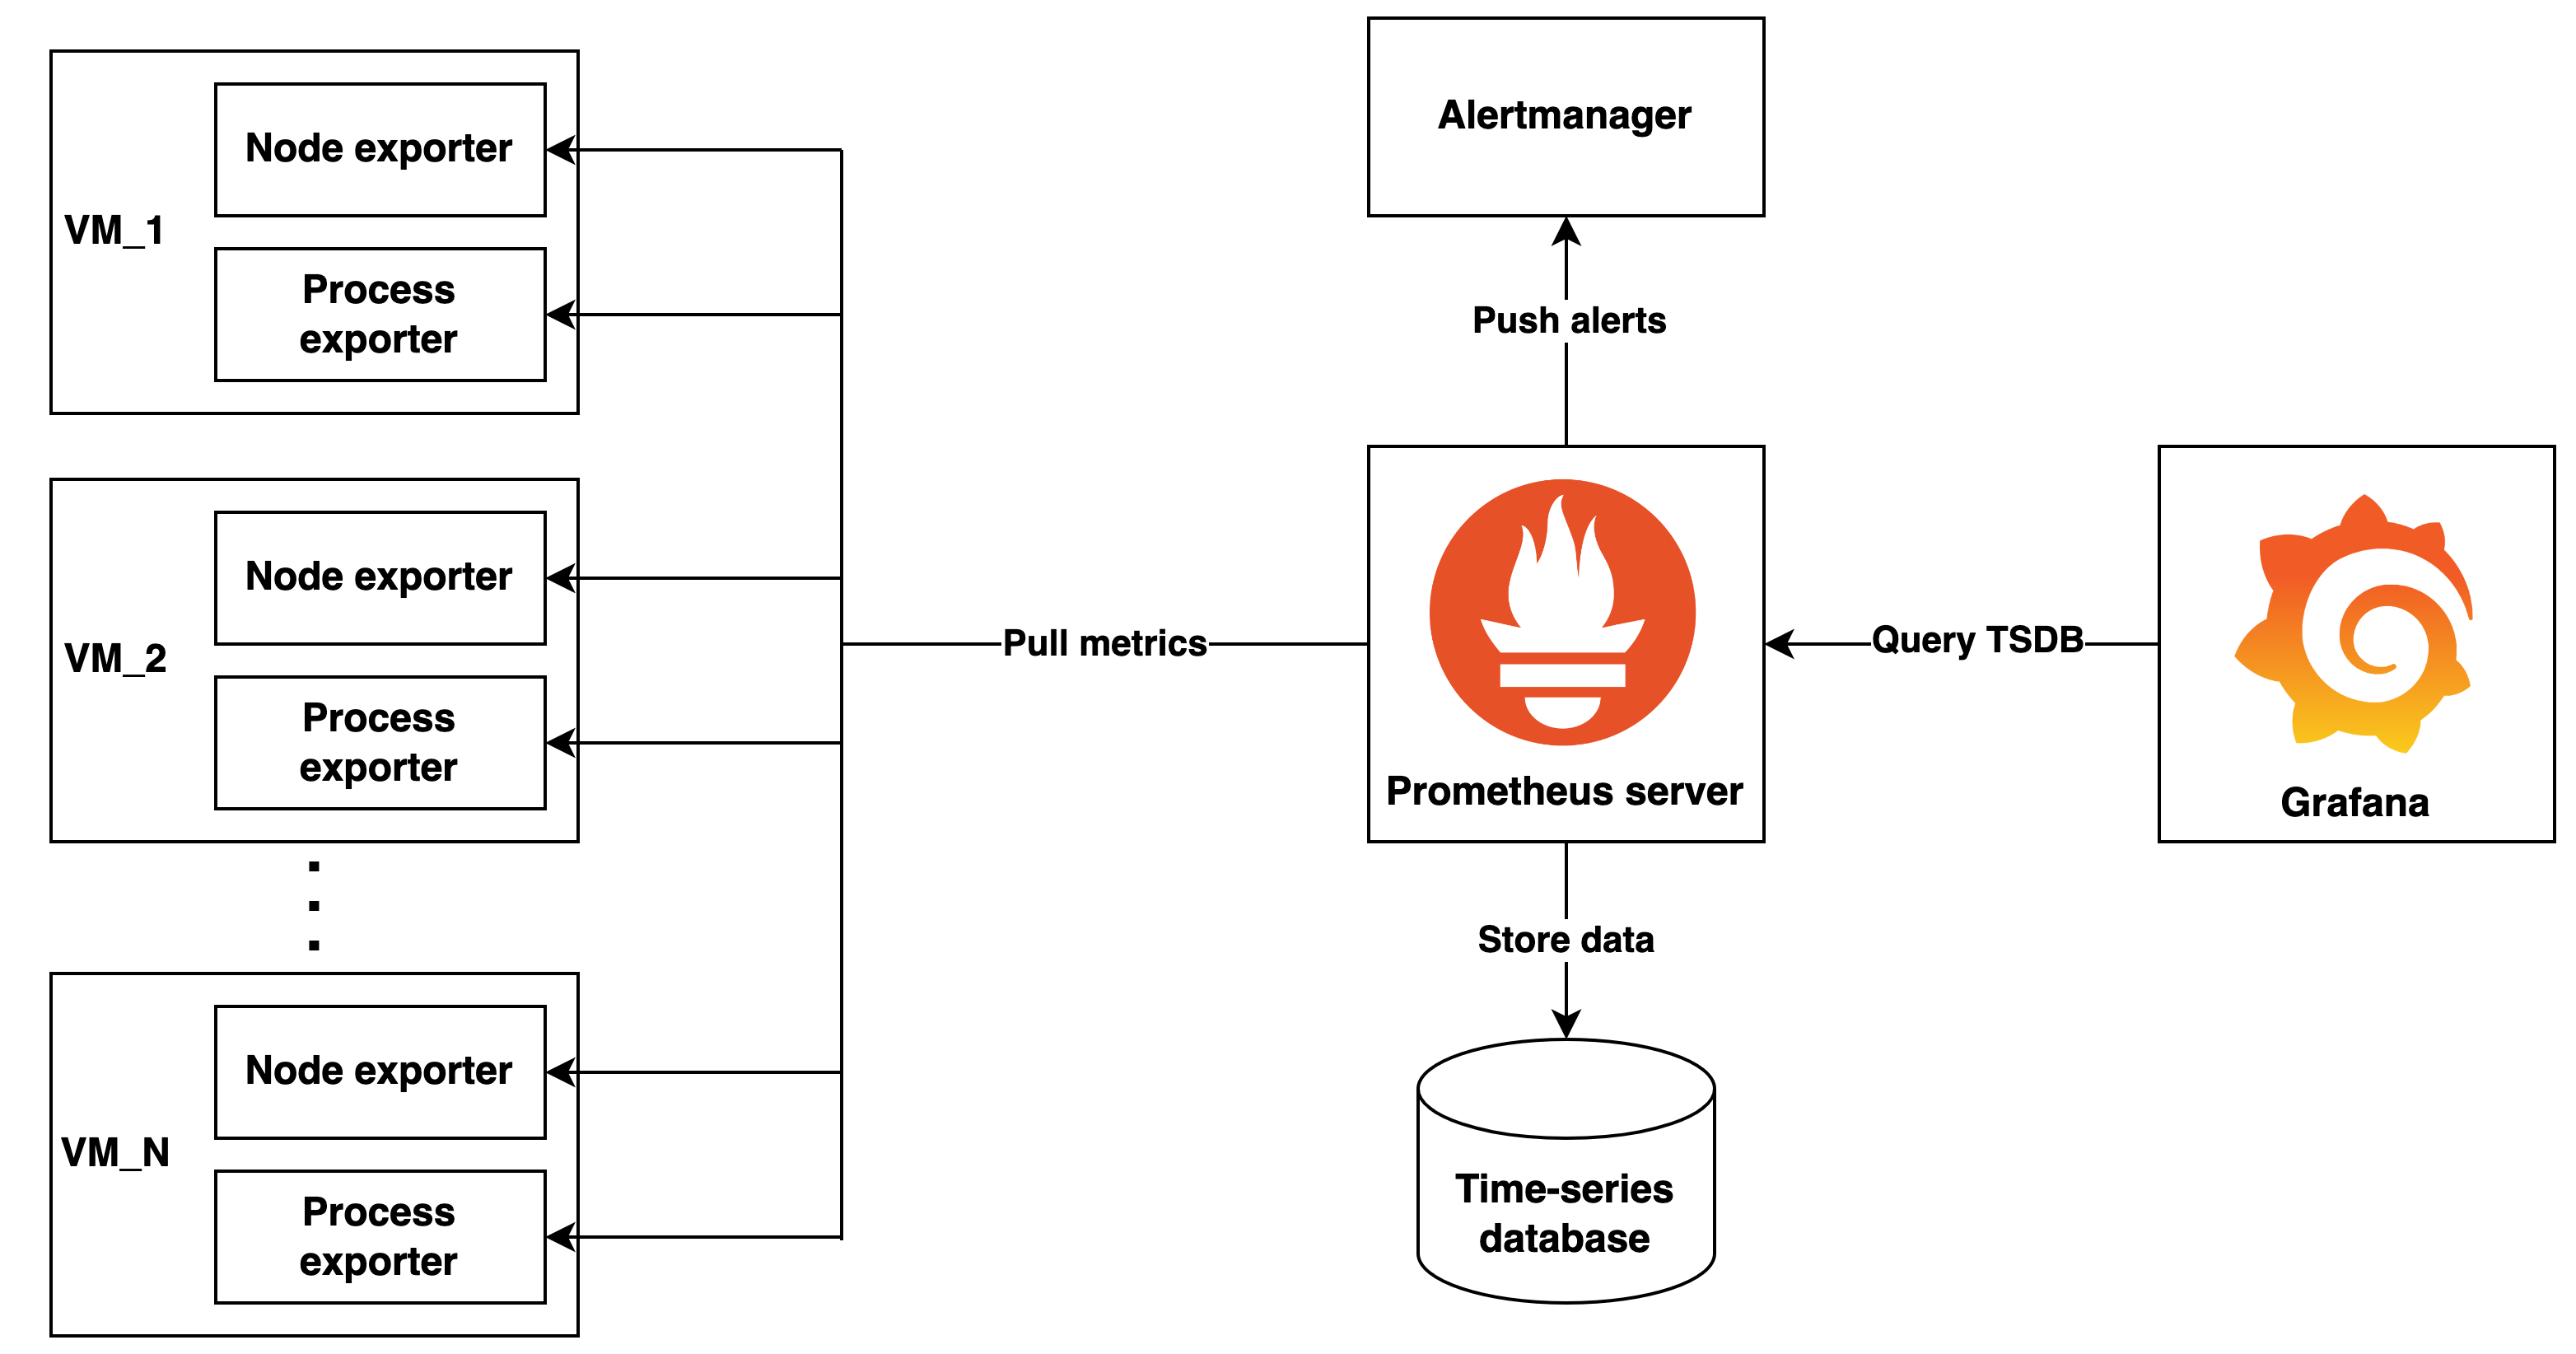
\includegraphics[width=1\linewidth]{images/prometheus.png}
  \caption{Standard Prometheus architecture for system performance metrics collection}
  \label{fig:prometheus}
\end{figure}

An example of how these metrics can be used for ``day 2 operations" is the one put in place by the \textbf{Krateo Composable FinOps} component \cite{krateo_docs}.
In this case, the system uses a set of Prometheus exporters and scrapers, configured through Kubernetes Custom Resources, to collect metrics about the VMs managed by the system.
The optimizations are encoded in a set of Kubernetes Custom Resources that are used by the specific operators (e.g., \textit{finops-operator-vm-manager}) to performs operations on the VMs, such as scaling up or down the VMs, stopping them during off-peak hours, etc \cite{krateo_docs}.
%Prometheus exporters (https://prometheus.io/docs/instrumenting/exporters/) + Prometheus scrapers for data collection.
%Generic Prometheus exporters and scrapers already used for Krateo Composable FinOps leveraging specific K8s Custom Resources. These exporters are generic and can scrape arbitrary metrics configured in specific CRs (for instance, collecting VMs CPU consumption though Azure APIs).
%From the Krateo Composable FinOps document: 
%- “we transform all optimizations into a set of Kubernetes Custom Resources (CRs) to act upon newly found cost-related deficiencies. This allows us to use Kubernetes operators (explicitly coded to interact with cloud services) to monitor these metrics and act automatically to apply changes to remote resources.”
%- “forward the optimization to the Krateo operator that manages the services that need to be optimized, for example, the Azure Operator to modify the size of a Virtual Machine;”
%- “the optimization is automatically encoded in a CR for the finops-operator-vm-manager, which then analyzes it and decides how to manage the Virtual Machine. For example, it could scale up or down the virtual machine, stop it for the night, etc.”
\newline

As Microsoft Azure documentation describes, there are actually two different categories of metrics that can be collected from a VM in the cloud: the \textbf{guest-level metrics} and the \textbf{hypervisor-level or host-level metrics} \cite{azure_vm_monitoring}.
The first category of metrics is collected by agents directly installed on the VMs, as described above.
The second category of metrics is collected by \textbf{cloud provider APIs}, and they provide information about the VMs from the hypervisor or host level.
For instance, in the case of Azure Virtual Machines, this date is related to the Hyper-V host that runs the VM \cite{azure_vm_monitoring}.
The difference between these two categories of metrics is that the guest-level metrics are more fine-grained and provide information about the actual resource usage of the VM (being collected at the OS level), while the hypervisor-level metrics are more high-level. \newline
%Azure monitoring REST API: https://learn.microsoft.com/en-us/azure/azure-monitor/essentials/rest-api-walkthrough?tabs=rest%2Cportal
%https://learn.microsoft.com/en-us/rest/api/monitor/metrics/list?view=rest-monitor-2023-10-01&tabs=HTTP
%https://learn.microsoft.com/en-us/azure/virtual-machines/monitor-vm 
To support the collection of metrics, several cloud providers offer agents that can be installed on the provider-specific VMs they manage.
One of the goal of these agents comparared to standard cloud-agnostic agents is to provide a more convenient experience for the user managing the VMs in the context of the cloud provider. 
Therefore these agents are usually more integrated with other cloud provider services and APIs.
In particular, we can cite the following agents: \textbf{Azure Monitor Agent} for Azure VMs, the \textbf{Google Ops Agent} for Google Compute Engine instances, and the \textbf{Amazon CloudWatch Agent} for AWS EC2 instances.
%Azure Monitor Agent (https://learn.microsoft.com/en-us/azure/azure-monitor/agents/azure-monitor-agent-overview)
%\textbf{Google Ops Agent}: “the primary agent for collecting telemetry from your Compute Engine instances” (https://cloud.google.com/monitoring/agent/ops-agent)
%Can be installed in various ways: manual installation, Usining Google Cloud Agent policies from glcoud CLI or using a configuration management tool like Terraform

\subsection{Power consumption metrics}

In the context of our use case, power consumption metrcis could be theoretically used to estimate the carbon footprint of a VM instance.
However, Public Cloud Providers do not provide real-time data about power consumption of a VM instance. \\

\textbf{Scaphandre} is an open-source monitoring agent designed to collect energy consumption metrics of a system \cite{scaphandre}.
Scaphandre represents a promising solution only for on-premises servers, as it relies on the Intel \textbf{Running Average Power Limit (RAPL)} sensors to collect power consumption data.
As a matter of fact, due to security and privacy concerns, public cloud providers do not expose to tenants the underlying RAPL sensors that Scaphandre relies on to track energy consumption \cite{scaphandre_github_issue}.
Therefore, Scaphandre is unsuitable for our current use case.

Another interesting and quite mature project is \textbf{Kepler} \cite{kepler}, which is a tool designed to monitor the energy consumption of Kubernetes resources (e.g., Nodes, Pods).
Being Kubernetes-centric, Kepler is not suitable for our first use case, as it does not provide real-time data about the power consumption of a generic VM instance.
However, Kepler could be potentially used in a future iteration of the system.

%manually estimate power consumption based on CPU utilization, memory usage. Could be a very difficult task. 
%there is the TEADS metodology like 

\subsection{Carbon metrics}
\label{sec:carbon_metrics}

As briefly mentioned in the beginning of this section, there is no adopted standard adopted by public cloud providers to calculate and expose the carbon footprint of a cloud resource.
In section \ref{sec:real_time_cloud}, we briefly described that the Green Software Foundation is working on a standard called \textbf{Real Time Cloud} that aims to provide a common standard for carbon footprint calculation.
The goal would be to have a \textbf{real-time carbon metric} to be used for optimization and that this metric would be added to the set of metrics that are already provided by the cloud providers (e.g., CPU usage, memory usage).
However, this standard is not yet adopted by any major public cloud provider which in turn provide only high-level monthly reports for carbon emission data.
A brief summary, as reported by one of the proposers of Real Time Cloud \cite{cloud_provider_sustainability_reports}, is shown in Table \ref{tab:cloud_carbon_emissions_reports}.

\begin{table}[t]
  \centering
  \renewcommand{\arraystretch}{1.2} % Increase row height for readability
  \setlength{\extrarowheight}{2pt} % Add extra space between rows
  \begin{tabularx}{\textwidth}{|X|X|X|X|X|X|}
  \hline
  \textbf{Cloud Provider}     & \textbf{Project name}                          & \textbf{Scope}            & \textbf{Geographical resolution} & \textbf{Carbon resolution} & \textbf{Time resolution} \\ \hline
  Amazon Web Services (AWS)   & AWS Customer Carbon Footprint Tool             & Account, EC2, S3, Other   & Continental                      & 0.001 Metric Tons of CO2e  & Monthly                  \\ \hline
  Microsoft Azure             & Azure Carbon Footprint API Schema              & Account, Service          & Country and region               & 0.001 Metric Tons of CO2e  & Monthly                  \\ \hline
  Google Cloud Platform (GCP) & Google Carbon Footprint BigQuery Export Schema & Account, Project, Service & Country, region and zone         & 0.1 Kilograms of CO2e      & Monthly                  \\ \hline
  \end{tabularx}
  \caption{Cloud provider sustainability reports}
  \label{tab:cloud_carbon_emissions_reports}
\end{table}
%Export Azure carbon optimization emissions data (Preview) (probably not fine-grained as we want)

We deem interesting to mention some of the existing projects that can be used to estimate the carbon footprint of a cloud resource.
\textbf{Cloud Carbon Footprint} \cite{cloud_carbon_footprint} is a tool that uses cloud provider billing (i.e., AWS Cost and Usage Reports with Amazon Athena, GCP Billing Export Table using BigQuery, Azure Consumption Management API) and resource usage metrics to provide an estimation of the carbon footprint of a cloud resource. For live grid carbon intensity an integration with Electricity Maps API is supported \cite{cloud_carbon_footprint}.
Another tool within the GreenOps ecosystem is the \textbf{Aether} calculation engine \cite{aether}
Currently only AWS and GCP are supported as it uses AWS CloudWatch and Google monitoring.
There is not the possibility to use a real-time Grid Carbon Intensity Coefficient since carbon data is extrapolated from “governative” data reports \cite{aether}.
A different approach to estimate the carbon footprint of resources, virtual machines in particular, is the one proposed by the \textbf{carbond} agent \cite{carbond:2023:hotcarbon}. 
This agent must be installed on the VM and aims to provide a real-time estimation of the carbon footprint of the VM via a file-system API \cite{carbond:2023:hotcarbon}.
It should be investigated further whether this agent could be used in cloud environments, since those settings, as described above, do not provide access to the underlying hardware sensors that are usually used by agents to estimate the power consumption of the VM.

%Example of a manual approach (not scalable due to tech specs research): https://devblogs.microsoft.com/sustainable-software/how-can-i-calculate-co2eq-emissions-for-my-azure-vm/ 
%The critical point here is to get/calculate the energy consumed by a cloud instance, since there are a huge number of technical configurations to find, retrieve and use for calculations.

\section{Multi-cloud resource management}
\label{sec:multi_cloud_resource_management}

The idea of a \textbf{dynamic management of workloads leveraging a multi-cloud paradigm} is not new. 
In this section we will provide an overview of some of the existing works in the literature that have tackled the problem of multi-cloud resource management.

\subsection{Dynamic Virtual Machine placement}
The work of Simarro et al. \cite{Simarro_2011} back at the dawn of cloud computing (2011) proposed a multi-cloud architecture for the dynamic placement of Virtual Machines (VMs).
The main objective of the system was cost optimization but this paradigm provides reliability and flexibility as well.
The scheduling part is comprised of a ``\textbf{cloud broker}" that is responsible for VM placement \textbf{transparent to users} providing a single uniform interface to the cloud resources.
Users can provide to the system a ``\textbf{service description template}'' to specify the number of VMs to provision and some constraints.
The cloud broker architecture is composed of two major components: the \textbf{scheduler} and the \textbf{cloud manager}. The former is responsible for placement decision across multiple cloud providers, while the latter is responsible for the actual management of the VMs in the cloud providers. More precisely, the cloud manager is represented by the OpenNebula (ONE) virtual infrastructure manager.
OpenNebula is an open-source platform that aims to provide a unified management interface for multiple virtualization technologies and cloud providers \cite{open_nebula}.

\subsection{Cloud service brokers}

Cloud service brokers (CSBs) were described and categorized by Wadhwa et al. \cite{Wadhwa_2013} in their work of 2013.
A CSB is a system that acts as an \textbf{intermediary} between cloud service providers and consumers, providing a \textbf{unified interface} to manage cloud resources across multiple providers.
The emerging market of cloud computing led to the proliferation of cloud services and providers, and by consequence the need for mechanisms to manage costs, capacity and resources. 
\newline

An interesting CSB example in the literature is the \textbf{STRATOS} system by Pawluk et al. \cite{STRATOS} proposed in 2012. 
The work can be considered a pioneer in the field of multi-cloud resource management since it can be framed in the first years of cloud computing but the proposed paradigms and concepts are relevant today.
STRATOS tried to \textbf{avoid the assumption of resource homogeneity} and represented an initial attempt to provide a ``\textbf{cross-cloud resource provisioning}'' system.
The proposed architecture enables the specification of high-level objectives that can be assessed in a standardized manner across different providers. The decision-making process is fully automated, shifting the decision point from deployment to runtime.
Users first submit a topology document, triggering the Cloud Manager to communicate with the Broker for topology instantiation. The Broker then conducts the initial resource acquisition decision, optimizing the allocation of resources across multiple providers (configured beforehand).
Experiments indicate that distributing workloads across different cloud providers can reduce the overall cost of the topology. The approach taken by the authors primarily focuses on two objectives: \textbf{cost efficiency} and \textbf{avoiding vendor lock-in}. The application environment was deployed on public cloud platforms, specifically AWS and Rackspace.
\newline

A more modern example of a similar strategy is the one developed at IBM and presented by Lublinsky et. al \cite{lublinsky2022kubernetesbridgeoperatorcloud}, denominated as ``\textbf{Kubernetes Bridge operator}'' in which the authors propose a system that allows to submit various types of workloads from Kubernetes to a \textbf{arbitrary external resource manager} .
In particular, they tackle the problem that not every workload can be deployed on Kubernetes and that especially scientific workloads might require specific and dedicated computing resources.
They refer, for instance, to \textbf{HPC clusters}, dedicated AI clusters, quantum computing cluster, etc.
Indeed they rely on the fact that specific resource managers (e.g., Slurm, IBM Spectrum LSF, IBM Quantum service, Ray, etc.) usually expose a \textbf{HTTP API}.
The proposed operator deploys Kubernetes Pods which in turn interact with external resource managers through HTTP APIs for job submission and monitoring.
Each Custom Resource, which represent the configuration of an external job, is associated with a specific Kubernetes Pod named ``Controller Pod'' (one per remote job) that is responsible for the interaction with the external resource manager (effectively acting as a proxy).
Credentials for external systems are stored in Kubernetes Secrets and are mounted in the Controller Pod.
In other words, the Bridge Operator is \textbf{generic and agnostic} and has the duty of managing Controller Pods which are are specifically tailored for a particular external resource manager.
The authors also provide an exemplificative set of implementations of controllers in the form of container images to be used in the Controller Pods.

\subsection{AI-based resource management in cloud computing}
\label{sec:ai_based_resource_management}

More recent works have focused on the development of systems that leverage AI techniques for the optimization of resource management in cloud computing environments.

The work of 2022 by Khan et al. \cite{KHAN2022103405} provides a comprehensive review of the state of the art in the field of machine learning (ML)-centric resource management in cloud computing.
Although this works focuses on the cloud provider side (\textbf{i.e., resource management in data centers}), it provides some interesting insights that can be leveraged also at different levels of the cloud computing stack.
The authors highlight the fact that traditionally, only static policies were used for resource management in cloud computing, but the advent of ML techniques has enabled the development of more dynamic and adaptive resource management systems \cite{KHAN2022103405}. \newline
% maybe add some more insights from this work

Tuli et al. in their work of 2021 \cite{TULI2022111124} propose a system named \textbf{HUNTER} which stands for ``Holistic resoUrce
maNagemenT technique for Energy-efficient cloud computing using aRtificial intelligence''. 
In this work, tasks are modeled as \textbf{containers instances}.
From a infrastructural point of view, the system is composed of four main components:
\begin{itemize}[itemsep=0.2pt, topsep=1pt]
    \item[$\bullet$] \textbf{Cloud Workload Management Portal}: a web-based portal that allows users to submit their workloads and specify the requirements (e.g., SLA constraints, QoS constraints, etc.).
    \item[$\bullet$] \textbf{Workload Manager}: responsible for the processing of incoming workloads.
    \item[$\bullet$] \textbf{Cloud Broker}: responsible for the allocation of resources to cloud worker nodes
    \item[$\bullet$] \textbf{Cloud Hosts}: set of cloud worker nodes, in the form of both private and public cloud.
\end{itemize}
The Cloud Broker is the core of the system and is further divided into three sub-managers: Service Manager, Cloud Data Centers Manager (CDC Manager), and Resource Manager.
The Service Manager is responsible for SLAs and QoS constraints, the CDC Manager is responsible for the actual allocation (provisioning) and migration of resources to cloud worker nodes and resource monitoring and the Resource Manager is responsible for the scheduling of tasks and contains the actual sustainability models (e.g., energy, thermal, cooling.).

\subsection{Policy-driven resource management systems}

García García et al. (2014) propose \textbf{Cloudcompaas} \cite{GARCIAGARCIA20141}, a Service Level Agreement (SLA)-driven platform for dynamic cloud resource management, focusing on the automation of resource provisioning, scheduling, and monitoring.
The aim of the work is to provide a SLA-aware Platform-as-a-Service platform for the entire management of the cloud resource lifecycle \cite{GARCIAGARCIA20141}.
The targeted resource to be managed spans from IaaS to PaaS and SaaS.
Their approach leverage the WebService-Agreement specification, a standard for SLA negotiation in web services, to define the SLA between the cloud provider and the cloud consumer.
Leveraging this representation, they propose a SLA-driven architecture with three main components: the \textbf{SLA Manager}, the \textbf{Orchestrator}, and the \textbf{Infrastructure Connector}.
The SLA Manager is the entry point for users and essentially builds and register agreements starting from the user requirements.
The Orchestrator, having a complete view of all the available cloud backends, performs the critical task of scheduling and resource allocation, considering the SLA constraints.
The Infrastructure Connector is the component that actually interacts with the cloud providers, performing the actual resource allocation and deallocation (provisioning and deprovisioning).
An interesting feature of the Infrastructure Connector is the ``configuration step'' in which arbitrary actions can be performed such as the \textbf{injection of a monitoring agent on a virtual machine}.
\newline

In the context of serverless computing environments, the work of 2021 by Mampage et al. \cite{9499407} proposes a deadline-aware dynamic resource management system.
The focus of the research is on both the provider and the consumer perspective, proposing a placement policy and ``dynamic resource management policy" that aims to minimize the cost of the provider while meeting the requirement of the consumer (i.e., the \textbf{deadline}).
\newline


%[Policy-Based Cloud Management Through Resource Usage Prediction]
% https://link.springer.com/chapter/10.1007/978-3-319-13464-2_14

%---

% Optimizing Cost and Maximizing Profit for Multi-Cloud-Based Big Data Computing by Deadline-Aware Optimize Resource Allocation
% https://link.springer.com/chapter/10.1007/978-981-15-8469-5_3

\section{Carbon-aware systems for resource management}
\label{sec:carbon_aware_resource_management}

Having provided an overview of the existing works in the field of multi-cloud resource management and having introduced the GreenOps landscape, we now focus on the state of the art in the field of carbon-aware resource management.
In particular, implementation choices and design patterns that can be leveraged for the development of a carbon-aware resource management system will be discussed.
\newline

The work by Sukprasert et al. \cite{10.1145/3599733.3606301} is a comprehensive analysis on the limits and benefits of the employment of geographical shifting and time shifting for cloud workloads.
The authors highlight the fact that different workloads have different characteristics and therefore different degrees of flexibility. Those include, for instance: \textbf{execution deadlines}, \textbf{data protection laws}, and \textbf{latency requirements}. Therefore, carbon savings are constrained by a complex set of factors that need to be taken into account when designing a carbon-aware system.

The following sections will present systems that have been developed by various research groups to tackle the problem of carbon-aware resource management in cloud computing environments.

%Bringing Carbon Awareness to Multi-cloud Application Delivery

\subsection{CASPER}

CASPER (Carbon-Aware Scheduling and Provisioning for Distributed Web Services) is a carbon-aware scheduling and provisioning system whose primary purpose is to minimize the carbon footprint of distributed web services \cite{Souza_2023}.
The system is defined as a multi-objective optimization problem that considers two factors: the \textbf{variable carbon intensity} and the \textbf{latency constraints} of the network.
By evaluating the framework in real-world scenarios, the authors demonstrate that CASPER achieves significant reductions in carbon emissions (up to 70\%) while meeting application \textbf{Service Level Objectives (SLOs)}, highlighting its potential for practical implementation in large-scale distributed systems.
The authors of CASPER highlight the importance of considering the workload characteristics such as memory state, \textbf{latency} and \textbf{regulatory constraints such as GDPR}.
The system is not adopting time-shifting since it is dealing with web services that are by their nature non-stopping workloads. The architecture is tied to scheduling Kubernetes resources inside Kubernetes clusters and does not consider external resource management.
%https://github.com/carbonfirst/casper?tab=readme-ov-file
%[HOW is it deployed]

\subsection{CASPIAN}

A research on carbon-aware scheduling in Kubernetes environments was conducted by the authors of CASPIAN (A Carbon-aware Workload Scheduler in Multi-Cluster Kubernetes Environments) \cite{10786568}.
The proposed system leverages Multi Cluster App Dispatcher (MCAD), a multi-cluster management platform, to provision workloads over distributed Kubernetes clusters.
Caspian is a scheduling and placement controller which lives in a master cluster and interacts with the MCAD to provision workloads across multiple geographical distributed clusters.
In particular, two main components are described: the \textbf{carbon tracker} and the \textbf{scheduler}.
The carbon tracker is responsible for the periodic collection of carbon intensity data along with worker cluster locations.
The scheduler, taking into account cluster information (i.e., carbon intensity, power efficiency, etc.), and workload requirements (e.g, \textbf{run time}, \textbf{deadline}, etc.), is responsible for the scheduling time and geographical placement of the workloads.

\subsection{CarbonScaler}

The work by Hanafy et al. \cite{10.1145/3626788} proposes a system that leverages the elasticity of batch cloud workloads to optimize carbon efficiency .
The targeted workloads are for instance \textbf{MPI jobs} and \textbf{Machine Learning training jobs}.
The system is entirely Kubernetes-based and it is composed of three main components: the \textbf{Carbon Profiler}, the \textbf{Carbon AutoScaler}, and the \textbf{Carbon Advisor}.
The Carbon Profiler main duty is to estimate energy usage of jobs.
The Carbon AutoScaler component is the core of the system and is a Kubernetes controller that leverage the \textbf{Kubeflow training operator}.
Kubeflow is effectively used for the resource management of batch jobs.
Finally, the Carbon Advisor simulates jobs execution in different configuration and allow the carbon reduction estimation.

\subsection{A Low Carbon Kubernetes Scheduler}
\label{sec:low_carbon_k8s_scheduler}

The work is focused on the extension of the Kubernetes scheduler (``kube-scheduler'') for the ranking and filtering of the ``greenest'' region for the deployment of entire Kubernetes clusters \cite{low_carbon_k8s_scheduler}.
The system is tailored and tested on Azure but can be extended to other cloud providers.
Provisioning  operations of the clusters are done by the system leveraging Kubernetes API or IaaS management APIs.
Therefore Kubernetes is leveraged as a control plane to provision other Kubernetes clusters.
An interesting feature proposed is the use of local air temperature and solar irradiance as tiebreaker for two datacenters with a similar carbon intense grid. 
The claim is that the solar irradiance has a bigger spread than the carbon intensity across global regions and that the local air temperature surrounding a datacentre affects the amount of energy needed for cooling. 

\subsection{Microsoft's Carbon-Aware Kubernetes strategy}
\label{sec:microsoft_carbon_aware_k8s}

Microsoft proposes a simple carbon-aware strategy for Kubernetes \cite{microsoft_carbon_aware_k8s}, integrating carbon intensity data into the scheduling process of Kubernetes Pods.
The Kubernetes scheduler, which allows custom rules for assigning nodes to pods, can incorporate carbon metrics like the Marginal Operating Emissions Rate (MOER) as factors in placement decisions. 
A weighted distribution can be created by normalizing the MOER values across the available Nodes.
These weightings are encoded in a YAML file and applied as a priority for the Scheduler, which out-of-the-box supports these kind of custom rules to extend the scheduling process.
The claim is that by combining three elements (i.e., Kubernetes scheduler, carbon intensity data, and a weighting algorithm) any Kubernetes instance can be made carbon-aware, at least in a simplified way.

\newpage

\section{Multi-cloud resource management - major outcomes}
\label{sec:multi_cloud_resource_management_outcomes}

%many simulation compared to real-world scenarios
%no much flexibility for what concern variaty of resource managed
%usually tied to one type of resource (e.g., VMs, K8s pods)
%usually either time shifting or geographical shifting
Many of the concepts described in this chapter are leveraged in the design and implementation of our system. 
We can briefly list some of the major recurrent elements that are generally needed in order to build a system for multi-cloud resource management:
\begin{enumerate}
    \item Representation of a generic workload
    \item Representations of constraint and objectives (e.g., SLAs, QoS)
    \item Cloud service broker / Orchestrator
    \item Modules to directly interact with the cloud providers
\end{enumerate}

\subsection{Differences with respect to the state of the art}

In the system proposed by this thesis, the elements needed for multi-cloud resource management (listed in the above section) are represented by \textbf{cloud-native components} in the Kubernetes ecosystem as described in the following chapters and as shown in Table \ref{tab:components_mapping}.

\begin{table}[t]
  \centering
  \renewcommand{\arraystretch}{1.3} % Adjust row height for readability
  \begin{tabularx}{\textwidth}{| l | X |} % 'X' makes the second column auto-wrap
    \hline
    \textbf{Generic component} & \textbf{Candidate solution} \\
    \hline
    Representation of a generic workload & Krateo CompositionDefinition \\
    \hline
    Representations of constraint and objectives (e.g., SLAs, QoS) & Open Policy Agent policies \\
    \hline
    Cloud service broker / Orchestrator & Krateo composition-dynamic-controller with Helm templating engine \\
    \hline
    Modules to directly interact with the cloud providers & Kubernetes operators of cloud providers \\
    \hline
  \end{tabularx}
  \caption{Mapping of main generic components for multi-cloud resource management to the components of the system proposed in this thesis}
  \label{tab:components_mapping}
\end{table}

From a general standpoint, the system proposed in this thesis is different from the state of the art analyzed for a number of reasons.
First of all, the system was designed to be easily integrated in a production environment rather than be used in a ``sandboxed" or simulation environment.
The system is designed to be \textbf{flexible} and \textbf{agnostic} with respect to the type of resources managed and the cloud providers used.
On the other hand, the works described in sections \ref{sec:multi_cloud_resource_management} and  \ref{sec:carbon_aware_resource_management} are usually tied to one type of resource (e.g., VMs, K8s pods) or when they are not, like in the case of the ``Kubernetes Bridge operator" \cite{lublinsky2022kubernetesbridgeoperatorcloud}, a specific controller must be implemented each time for each external resource manager.
In our case, we leverage Kubernetes as a control plane to manage the resources of the cloud providers.
We do not need to implement a specific controller for each cloud provider but we leverage the Kubernetes ecosystem of operators to manage cloud resources.
We then leverage Open Policy Agent and the ``Policy as Code'' paradigm to encode the constraints and objectives of the system, which we believe is a more flexible and powerful approach than the one used in the works described in the previous sections.

\newpage
